\section{Systems with Similar Instability Problems}
\graphicspath{{figures/"Preanalysis&Requirement"/SimilarSystems/}}

In order to stabilize the rocket in flight, a controller must be implemented to correct the rockets trajectory deviation during flight.

The possibility of damaging the rocket or the controller needs to be countered by the efficiency of the control system.


Experimenting such a system during flight is expensive and presents nonnegligible hazards.
Is there a system that has similar instability properties of rockets, and presents fewer restrictions to experiment?

The Cubli is a system known for its instability. It is commonly used in Control Theory to analyze the behavior of a reaction of a wheel inverted system. The advantages of the usage a Cubli is its ability to reach its equilibrium position in microgravity environments, such as asteroids. This is not relevant for a rocket instability project. And can therefore not be directly related to the instability of a rocket.

A recent technology facing instability is Segway. A Segway is an application of an inverted pendulum to a two wheeled self-balance vehicle. The objective is to detect and stabilize the instability of the vertical stick to move the vehicle and prevent the user to fall. This vehicle requires three body directions instead of the linear motion of an inverted pendulum. The study of instability properties of a Segway system would mean the study of elements nonexistent or negligible in a rocket system.

An inverted pendulum objective is to stabilize a stick whose center of mass is above pivot point. The process is done using a horizontal force, resulting in a first degree of freedom rotation, as found in a rocket system. A double inverted pendulum is a combination of an inverted pendulum and a double pendulum. The stability of the stick is reached by applying a torque between the two pendulums.
%\begin{figure}[htbp]
%	\centering
%	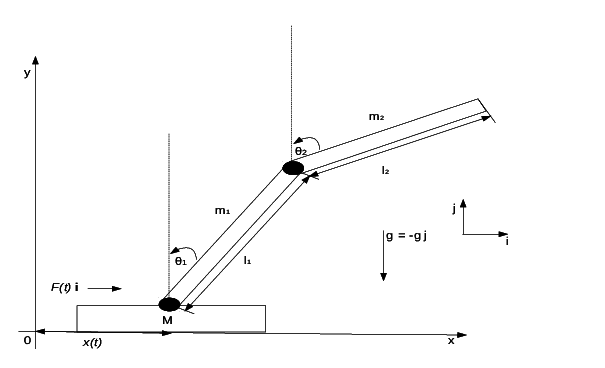
\includegraphics[width=0.6\linewidth]{double-inverted-pendulum}
%	\caption{Summary of forces applied to a double inverted pendulum. The process is equivalent to figure  \vref{fig:RocketForceSummary}.}
%	\label{fig:DoubleInvertedPendulum}
%\end{figure}

In consideration of the different applications and similarities of the three systems, the double inverted pendulum will be further analyzed. The objective is to model the dynamics of both the double inverted pendulum and the rocket, and then compare and relate the models to determine similarities. This should lead to designing a control system for stabilizing the inverted pendulum, which could be implemented on the rocket as a stabilization control system. 



